\documentclass[tikz,border=15pt]{standalone}
\usepackage{helvet}
\usepackage{amsmath}
\renewcommand{\familydefault}{\sfdefault}
\usetikzlibrary{automata, positioning, arrows.meta, shapes.geometric, calc}

\definecolor{emeraldpine}{HTML}{1A4D3E}
\definecolor{ethbronze}{HTML}{B87333}
\definecolor{harvardcrimson}{HTML}{A51C30}
\definecolor{paleink}{HTML}{A0AEC0}
\definecolor{ethdarkblue}{HTML}{1F407A}
\definecolor{ink}{HTML}{1A202C}
\definecolor{cardbg}{HTML}{F8FAFC}
\definecolor{softink}{HTML}{4A5568}

\begin{document}
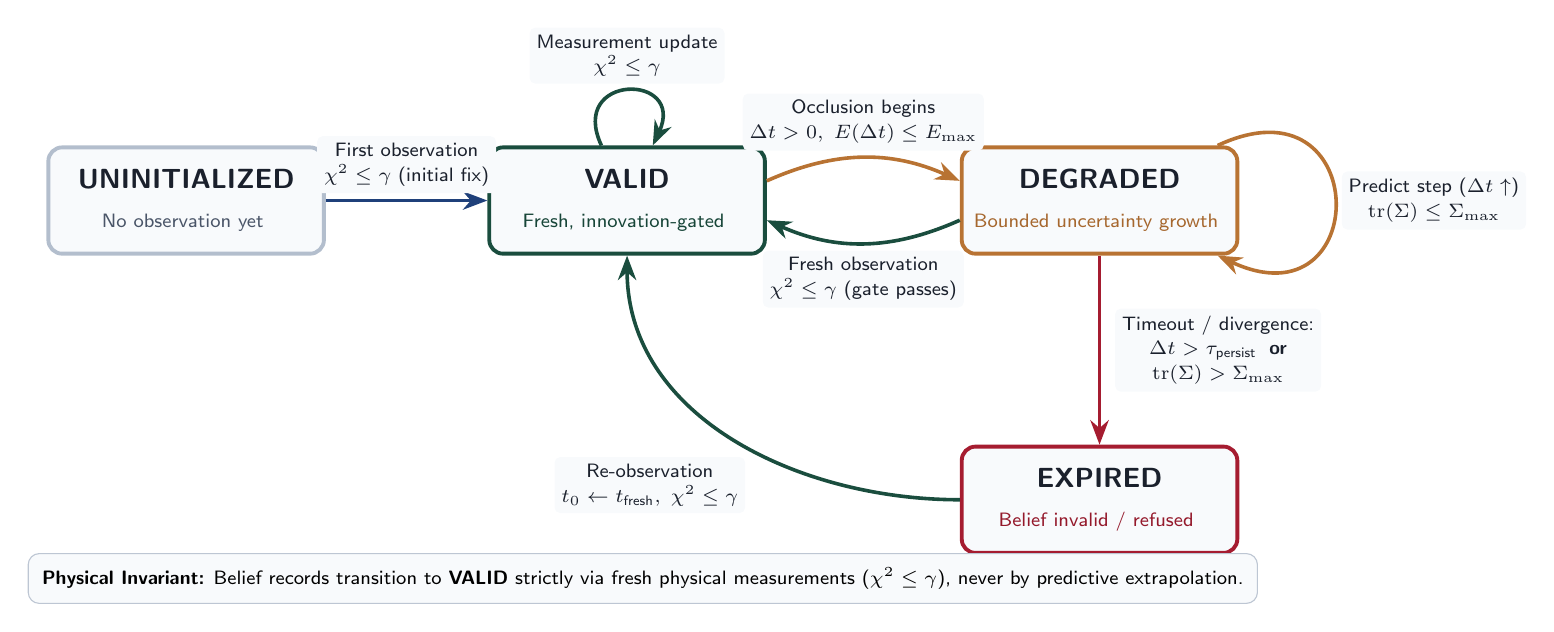
\begin{tikzpicture}[
    >=Stealth,
    font=\sffamily,
    state/.style={
        rectangle, 
        rounded corners=5pt, 
        draw=#1, 
        fill=cardbg, 
        line width=1.4pt,
        minimum width=3.5cm, 
        minimum height=1.35cm, 
        align=center, 
        text=ink
    },
    arr/.style={->, thick, ethdarkblue, line width=1.3pt},
    arr-green/.style={->, thick, emeraldpine, line width=1.3pt},
    arr-red/.style={->, thick, harvardcrimson, line width=1.3pt},
    arr-amber/.style={->, thick, ethbronze, line width=1.3pt},
    lbl/.style={font=\sffamily\scriptsize, text=ink, align=center, fill=cardbg, inner sep=2.5pt, rounded corners=2pt}
]

% Nodes
\node[state=paleink!80] (uninit) at (0, 0) {
    \textbf{UNINITIALIZED}\\[2pt]
    \fontsize{7.5pt}{9pt}\selectfont\color{softink} No observation yet
};

\node[state=emeraldpine] (valid) at (5.6, 0) {
    \textbf{VALID}\\[2pt]
    \fontsize{7.5pt}{9pt}\selectfont\color{emeraldpine!90!black} Fresh, innovation-gated
};

\node[state=ethbronze] (degraded) at (11.6, 0) {
    \textbf{DEGRADED}\\[2pt]
    \fontsize{7.5pt}{9pt}\selectfont\color{ethbronze!90!black} Bounded uncertainty growth
};

\node[state=harvardcrimson] (expired) at (11.6, -3.8) {
    \textbf{EXPIRED}\\[2pt]
    \fontsize{7.5pt}{9pt}\selectfont\color{harvardcrimson!90!black} Belief invalid / refused
};

% Transitions
% 1. UNINIT -> VALID
\path[arr] (uninit) edge node[above, lbl, yshift=2pt] {First observation\\[1pt]$\chi^2 \le \gamma$ (initial fix)} (valid);

% 2. VALID -> DEGRADED (Forward curved arrow)
\path[arr-amber] ($(valid.east)+(0,0.25)$) edge[bend left=24] 
    node[above, lbl, yshift=2pt] {Occlusion begins\\[1pt]$\Delta t > 0,\; E(\Delta t) \le E_{\max}$} ($(degraded.west)+(0,0.25)$);

% 3. DEGRADED -> VALID (Return curved arrow)
\path[arr-green] ($(degraded.west)+(0,-0.25)$) edge[bend left=24] 
    node[below, lbl, yshift=-2pt] {Fresh observation\\[1pt]$\chi^2 \le \gamma$ (gate passes)} ($(valid.east)+(0,-0.25)$);

% 4. DEGRADED -> EXPIRED (Downward arrow)
\path[arr-red] (degraded) edge 
    node[right, lbl, xshift=5pt] {Timeout / divergence:\\[1pt]$\Delta t > \tau_{\text{persist}}$ \;\textbf{or}\\[1pt]$\operatorname{tr}(\Sigma) > \Sigma_{\max}$} (expired);

% 5. EXPIRED -> VALID (Sweeping return curve)
\draw[arr-green] (expired.west) to[out=180, in=-90] 
    node[pos=0.45, below left, lbl, xshift=-2pt, yshift=-2pt] {Re-observation\\[1pt]$t_0 \leftarrow t_{\text{fresh}},\; \chi^2 \le \gamma$} (valid.south);

% Self-loops
\path[arr-green] (valid) edge[loop above, looseness=4, out=115, in=65] 
    node[above, lbl, yshift=2pt] {Measurement update\\[1pt]$\chi^2 \le \gamma$} (valid);

\path[arr-amber] (degraded) edge[loop right, looseness=4, out=25, in=-25] 
    node[right, lbl, xshift=2pt] {Predict step ($\Delta t \uparrow$)\\[1pt]$\operatorname{tr}(\Sigma) \le \Sigma_{\max}$} (degraded);

% Bottom invariant note
\node[fill=cardbg, draw=paleink!70, rounded corners=4pt, inner sep=5pt, font=\scriptsize, align=center] 
    at (5.8, -4.8) {\textbf{Physical Invariant:} Belief records transition to \textbf{VALID} strictly via fresh physical measurements ($\chi^2 \le \gamma$), never by predictive extrapolation.};

\end{tikzpicture}
\end{document}
